We have evaluated the coarse-grain parallelization implemented in 
the Caffe DNN framework. All exeperiments have been performaed 
in a 16-core Xeon E5-2667 at 3.30GHz with a NVIDIA K40 GPU. 
The machine run Red Hat Enterprise Linux Server release 6.6 (Santiago), 
and we have used the GCC compiler suite version g++ (GCC) 4.4.7 20120313 
(Red Hat 4.4.7-11). We configured the Caffe framework to use OpenBLAS 
for the implementation of basic linear algebra subsoutines. 
For the GPU programming, we have used cuda toolkit 7.0 and cuDNN. 
The datasets used for the evaluation are the MNIST and CIFAR-10 
image classifiers.

%\setlength{\textfloatsep}{3pt}

\begin{figure*}[]
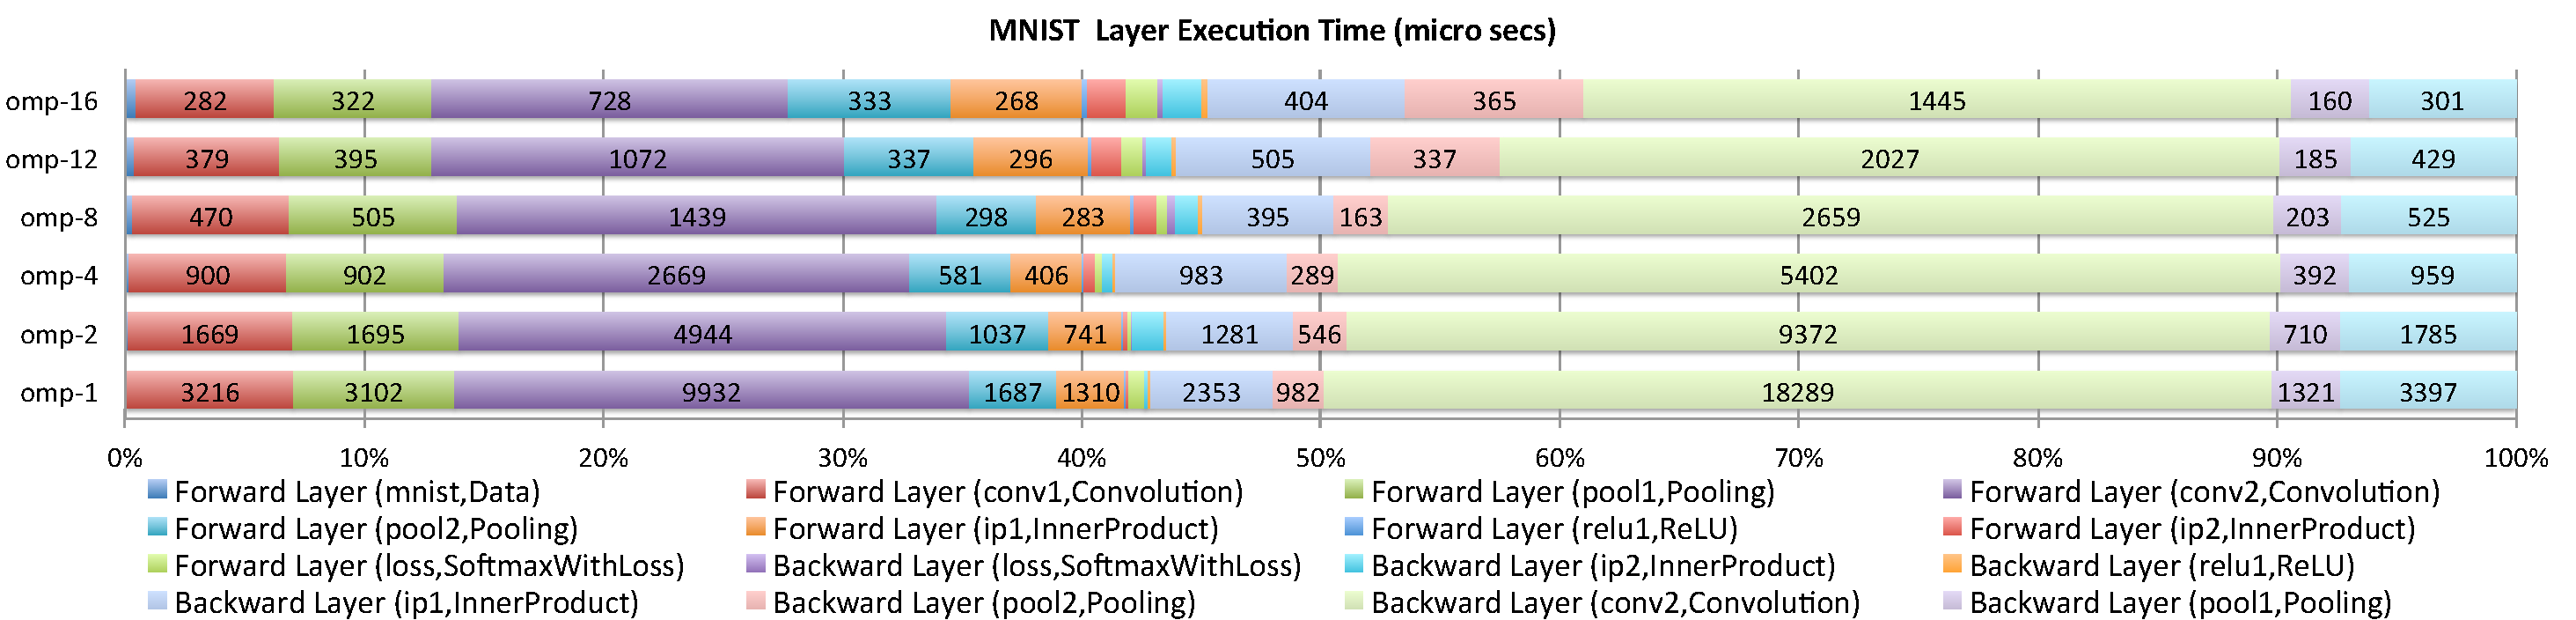
\includegraphics[width=\linewidth]{figures/mnist-rel-abs-time.pdf}
\caption{MNIST - Relative and absolute execution layer time for CPU executions. Layers in the legend are ordered from left-to-right in each horizontal bar. Horizontal bars correspond to the cases of 1, 2, 4, 8, 12 and 16 threads. All execution times are in microseconds.}
\label{fig-mnist-abs-rel}
\end{figure*}

\begin{figure*}[]
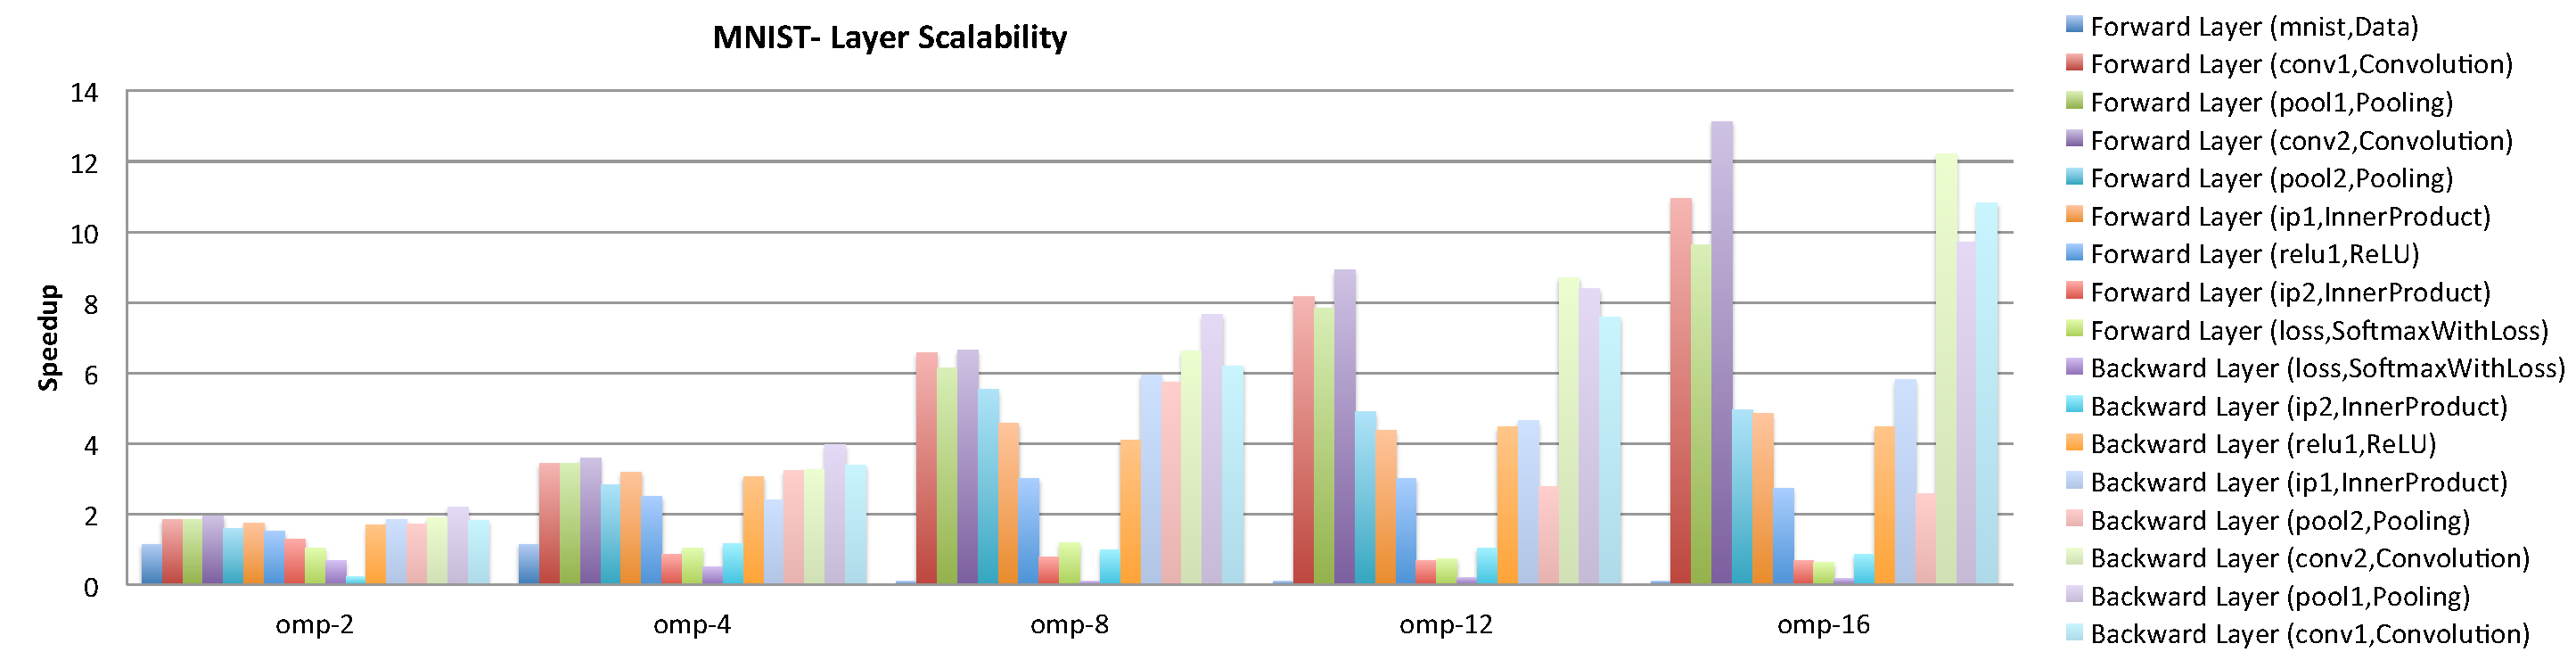
\includegraphics[width=\textwidth]{figures/mnist-scalability-layer.pdf}
\caption{MNIST - Layer scalability for the CPU executions. Layers are identified as in the legend for Figure \ref{fig-mnist-abs-rel}. Layers in the legend are ordered from left-to-right in each cluster. Clusters correspond to the cases of 2, 4, 8, 12 and 16 threads. Y-axis measures speedup factors from the serial CPU execution.}
\label{fig-mnist-scalability}
\end{figure*}

\begin{figure*}[]
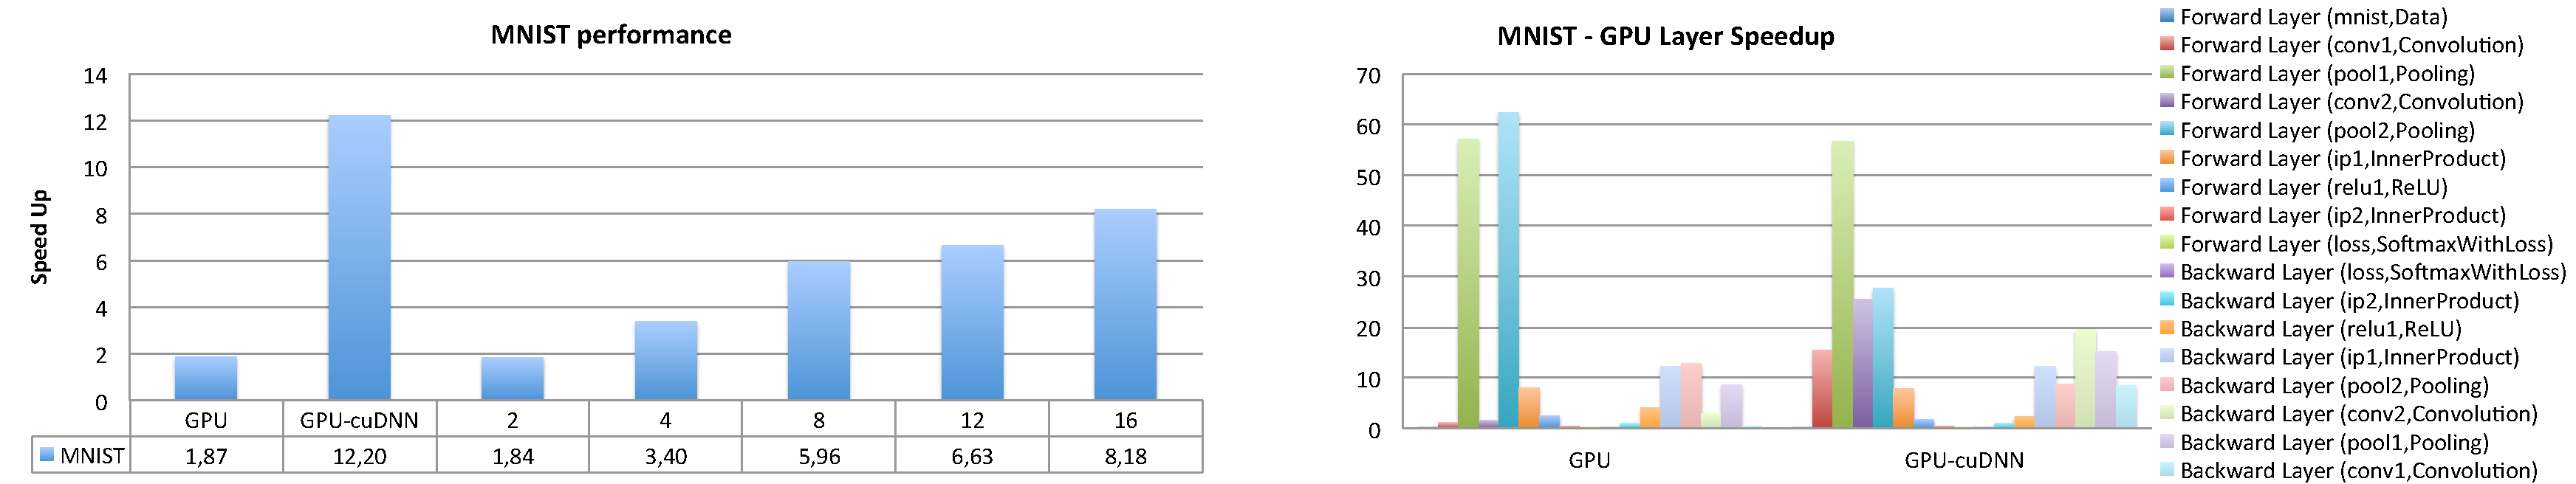
\includegraphics[width=\textwidth]{figures/mnist-abs-perf+gpu-layer.pdf}
\caption{MNIST - \textbf{Leftmost side}: Absolute speedup factors for OpenMP (2, 4, 8, 12 and 16 threads), plain-GPU and cuDNN-GPU versions. performance. \textbf{Rightmost} side: GPU layer scalability for plain-GPU and cuDNN-GPU versions. Layers are identified as in the legend for Figure \ref{fig-mnist-abs-rel}.}
\label{fig-mnist-overall}
\end{figure*}

\subsection{MNIST dataset}
For the performance analysis of the MNIST dataset we have first 
developed a per-layer study both coarse-grain and fine-grain parallelizations.For the coarse-grain case we identify what are the main limiting 
performance factors. Then we describe the overall performance of the 
coarse-grain parallelization. 

\subsubsection{Coarse-grain Layer Performance}
Figure \ref{fig-mnist-abs-rel} shows the absolute execution time per layer 
and the relative weight in the overall execution time. Horizontal bars 
correspond to executions with 1, 2, 4, 8, 12 and 16 threads. In general, 
two layers dominate the whole execution: the convolutional and pooling 
layers. No matter the number of threads, these two type of layers always 
account for almost 80\% of total execution time, adding their forward 
and backward passes. Notice that there are different instances of the 
same type of layer but with very different absolute execution time. 
For instance, the \emph{conv1} and conv2 layers, and in a smaller magnitude 
the pool1 and pool2 layers. After the convolutional and pooling layers, 
the next significant layer is the inner product ip1. The rest of layers, 
expose a very small contribution to the overall execution time 
(e.g.: loss, ReLU and ip2 layers in their forward and backward passes).
In general, notice that in each horizontal bar there is a zone where the 
work in each layer phase decreases. This corresponds to the center part, 
composed of the forward and backward passes of pool2, ip1, ReLU, ip2 and loss.
This behavior is associated to the dimensionality reduction that neural 
networks do, and affects the work granularity for the parallelization process.
Moreover, this behavior limits the overall scalability of the training process.

Figure \ref{fig-mnist-scalability} shows the scalability curve of each layer. 
We identify three layer behaviors. First, notice the u-shape of the 
scalability trends for any number of threads. The center points 
correspond to the layers that we have previously identified as not 
significant in the overall execution time (e.g.: loss, ReLU and ip2 layers). 
These layers do not scale at all, but they do not represent a limitation for 
the overall performance. The two sides on the center values correspond 
to the forward and backward passes of the rest layers. For these, we detect 
two types of layer behavior. 

Layers ip1 and pool2 present very poor scalability curves. 
For ip1, in both the forward and backward passes, the layer 
presents speedups of 4,58 and 5,93 for the forward and backward 
pass respectively and with 8 threads. The layer does not improve 
the speedup with more threads. The pool2 layer exposes the same 
behavior with maximum speedup of 5.52 and 5.73 with 8 threads in 
the forward and backward pass respectively. The reason for this 
behavior is two fold. First, notice the two layers are immediately 
stacked one on top of the other. This means that the 
output of the pool2 layer is the input for the ip1 layer. It happens 
that the blob shapes between the two layers do not match. The pool2 
layer is parallelized according to its input blob dimensions, and 
produces its output blob (input blob for ip1) following the resulting 
work and data distribution coming out from the parallelization. When 
it comes the execution of the ip1 layer, its parallelization is done 
according to its input blob dimensions (output blob of pool2), which do 
not match those of the input blob for the pool2 layer. Thus, theres is 
an unavoidable lost of locality for the execution of the ip1 layer. 
Second, both layers suffer from a poor granularity when executing with 
more than 8 threads. In Figure \ref{fig-mnist-abs-rel} we observe that 
with more than 8 threads the forward and backward passes of the two layers 
are in the range of 350 microseconds.

Layers conv1, pool1 and conv2 present good scalability curves. They 
correspond to the layers in both sides of the center part of the 
scalability layer curves. In general, these layers respond well to the 
increments on the number of threads. This is explained by two factors. 
First, all these layers expose a considerable amount of work, as it has 
been indicated with Figure \ref{fig-mnist-abs-rel}. Second, all of them 
are stacked one next to each other within the network, and all of them 
match their input/output blob dimensions. Thus, data locality is 
preserved along the their execution in both the forward and backward passes.
We have detected that although being exactly the same layer, the conv1 
and conv2 layers have close to a 10\% difference in speedup. 
In particular, the conv2 layer exposes greater speedups than conv1. 
This happens more noticeably with more than 8 threads and for the 
forward pass. The difference between the two layers is the position 
they occupy in the layer stack. Conv1 is the immediate layer after the 
data layer in the MNIST network. The data layer is responsible for
feeding the network with data samples. The layer executes sequentially, 
so the data associated to all images generates a memory footprint that is 
not matching the one generated along the parallel execution of the 
conv1 layer. Therefore, the conv1 layer suffers from a poor data 
locality with its immediate previous layer.

%\begin{figure*}[]
%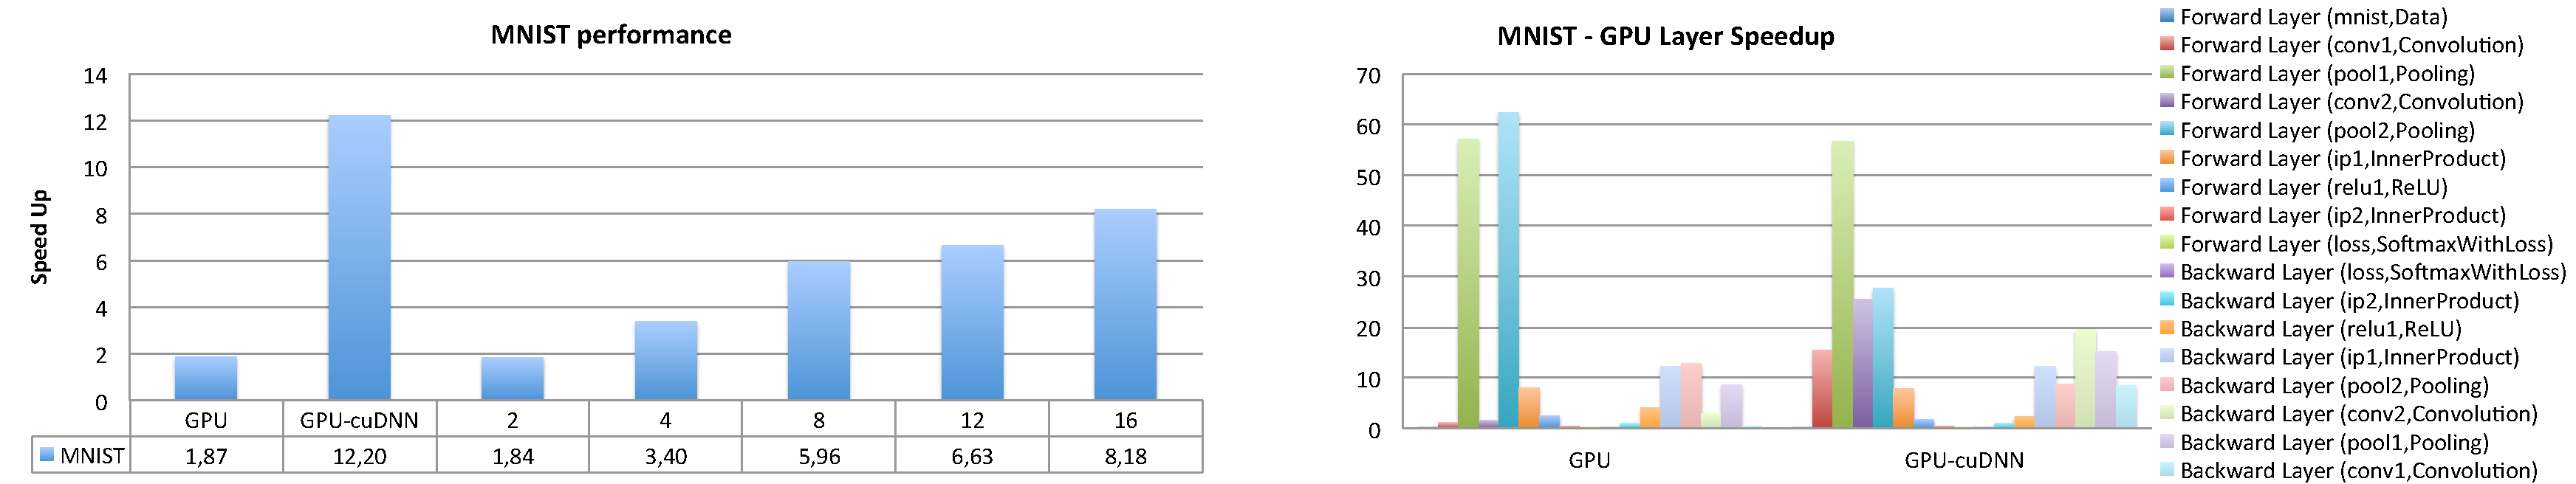
\includegraphics[width=\textwidth]{figures/mnist-abs-perf+gpu-layer.pdf}
%\caption{MNIST - \textbf{Leftmost side}: Absolute speedup factors for OpenMP (2, 4, 8, 12 and 16 threads), plain-GPU and cuDNN-GPU versions. performance. \textbf{Rightmost} side: GPU layer scalability for plain-GPU and cuDNN-GPU versions. Layers are identified as in the legend for Figure \ref{fig-mnist-abs-rel}.}
%\label{fig-mnist-overall}
%\end{figure*}

\subsubsection{Fine-grain Layer Performance}
The fine-grain layer parallelization is available in Caffe in two versions. 
All available layers come with a native GPU implementation of their 
forward and backward pass. We identify this version as the \emph{plain-GPU} 
version. Specifically for the convolutional and pooling layers, Caffe 
includes a cuDNN-based version. We identify this version as the 
\emph{cuDNN-GPU} version. 
%Both present similar execution time distribution 
%as the omp-1 serie in Figure \ref{fig-mnist-abs-rel}: convolutional and 
%pooling layers dominate the GPU execution. 
Rightmost side of Figure \ref{fig-mnist-overall} shows the per-layer 
speedup numbers for the plain-GPU and cuDNN-GPU versions. 
For the plain-GPU version, all layers present speedup below 
the 10$\times$ bar unless for specific exceptions. The pool1 and pool2 
layers expose extraordinary speedups of 57$\times$ and 62$\times$ for their 
forward passes respectively. The pool2 layer presents a speedup of 
12.81$\times$ in its backward pass and the ip1 layer is also above the 
10$\times$ bar with a speedup of 12.25$\times$ in its backward pass.
In contrast, the convolutional layers present a very poor speedup, with 
1.11, 1.63 for the forward passes of conv1 and conv2, and 0.43$\times$ and 2.86$\times$ 
in their respective backward passes. 

For the cuDNN-GPU, the results are similar, unless for the convolutional 
and pooling layers. The conv1 and conv2 layers experiment an extraordinary 
improvement reaching speedups of 15$\times$, 25$\times$, 19$\times$ and 8$\times$ in their 
forward and backward passes. In contrast, the pool2 layer experiments a 
dramatic loss of performance: it drops from 62$\times$ to 27$\times$ in its forward 
pass and from 12.81$\times$ to 8.81$\times$ in its backward pass. More moderately, 
the ReLU layer also suffers a performance drop from 2.47$\times$ to 1.74$\times$ and 
from 4$\times$ to 2,41$\times$ in its froward and backward passes respectively. 
In general, cuDNN corresponds to a case where the industry has deployed 
a highly optimized implementation of layer transformations that well 
understood and no longer in a research stage. In this situation, the 
fine-grain parallelism makes a difference, after the corresponding recoding 
efforts.

%\begin{figure}[b]
%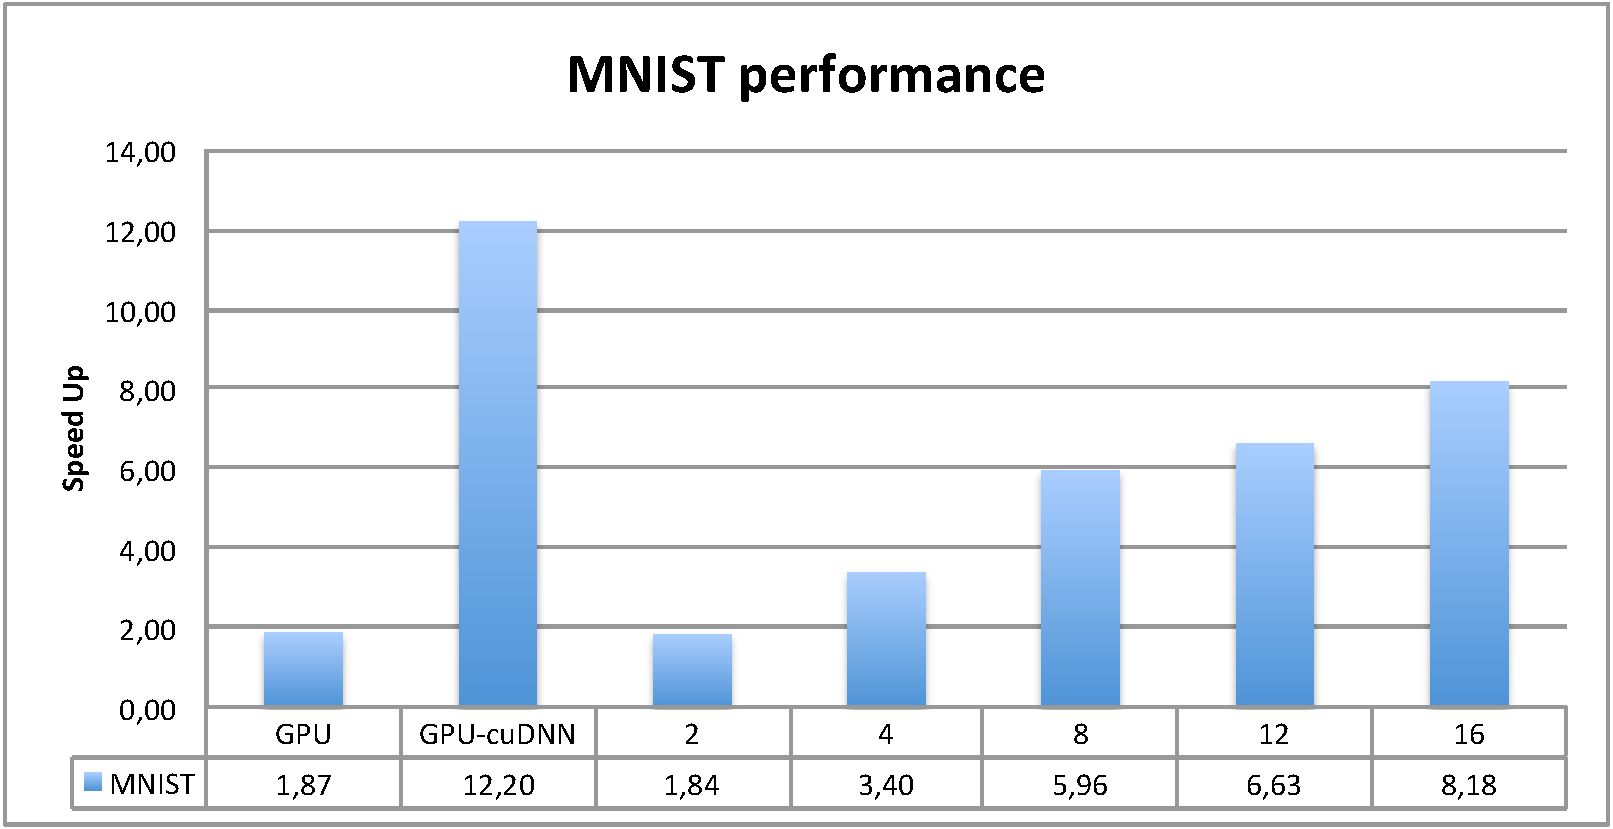
\includegraphics[width=\linewidth]{figures/mnist-abs-perf-all.pdf}
%\caption{\todo{CAPTION}}
%\end{figure}

\subsubsection{Overall Performance}
Figure \ref{fig-mnist-overall} shows the overall performance of
the coarse-grain parallelization and the fine-grain parallelization in 
its two versions GPU and GPU-cuDNN. The coarse-grain reaches a speedup 
close to a 6$\times$ with 8 threads, and 8$\times$ with 16 threads. The lack of 
the scalability for the CPU version is related to the poor scalability 
of fine-grained layers that when executing with 16 threads drag down 
the performance. In addition, we suspect the serial initialization of 
the network structures is giving a suboptimal memory allocation in 
the NUMA nodes. All of this is affecting the final scalability of 
the coarse-grain version. The fine-grain GPU version shows a 
modest speed up close to 2$\times$. The reason for this difference is related 
to the performance of the convolutional layers. In general, this version 
corresponds to a base line defined by the Caffe native implementation 
of the GPU acceleration. It represents a case for the performance the DNN 
community can obtain with a fine-grain parallelization and very significant 
coding efforts. Remember that within Caffe, all layers have to have 
both a CPU and GPU implementation to guarantee GPU acceleration. 
In conclusion, the coarse-grain approach minimizes the coding efforts 
and delivers better performance levels. Of course, when compared to 
the cuDNN case, the fine-grain approach makes a difference. 
It delivers a 12$\times$ speedup. But solutions like the cuDNN framework are 
only available when the layer types and their implementation have become 
a product and are no longer in a research stage. Thus, they can have a 
highly optimized implementation. For a DNN framework like Caffe, 
which is aimed to give support for research in new network architectures 
with novel layer types, the fine-grain parallelism imposes hard recoding 
efforts. In contrast, the coarse-grain option is much more immediate and 
effective.

\begin{figure*}[]
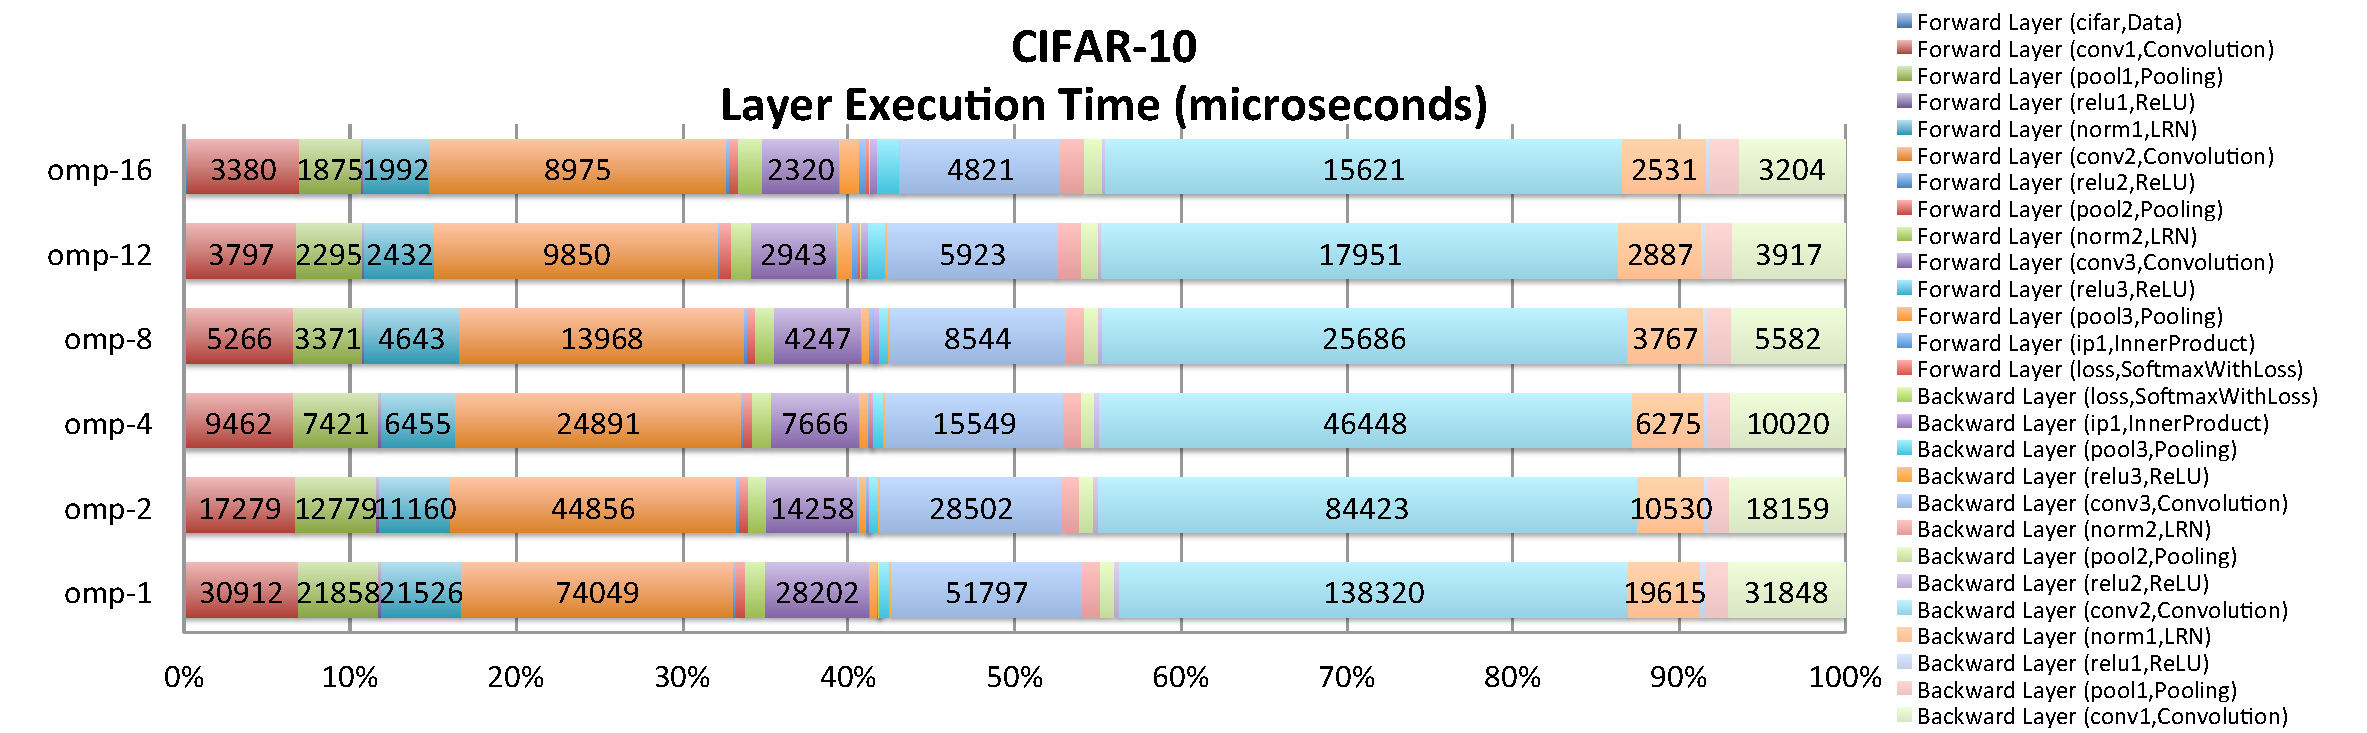
\includegraphics[width=\textwidth]{figures/cifar-abs-rel-time.pdf}
\caption{CIFAR-10 - Relative and absolute execution layer time for CPU executions. Layers in the legend are ordered from left-to-right in each horizontal bar. Horizontal bars correspond to the cases of 1, 2, 4, 8, 12 and 16 threads. All execution times are in microseconds.}
\label{fig-cifar-abs-rel}
\end{figure*}

\begin{figure*}[]
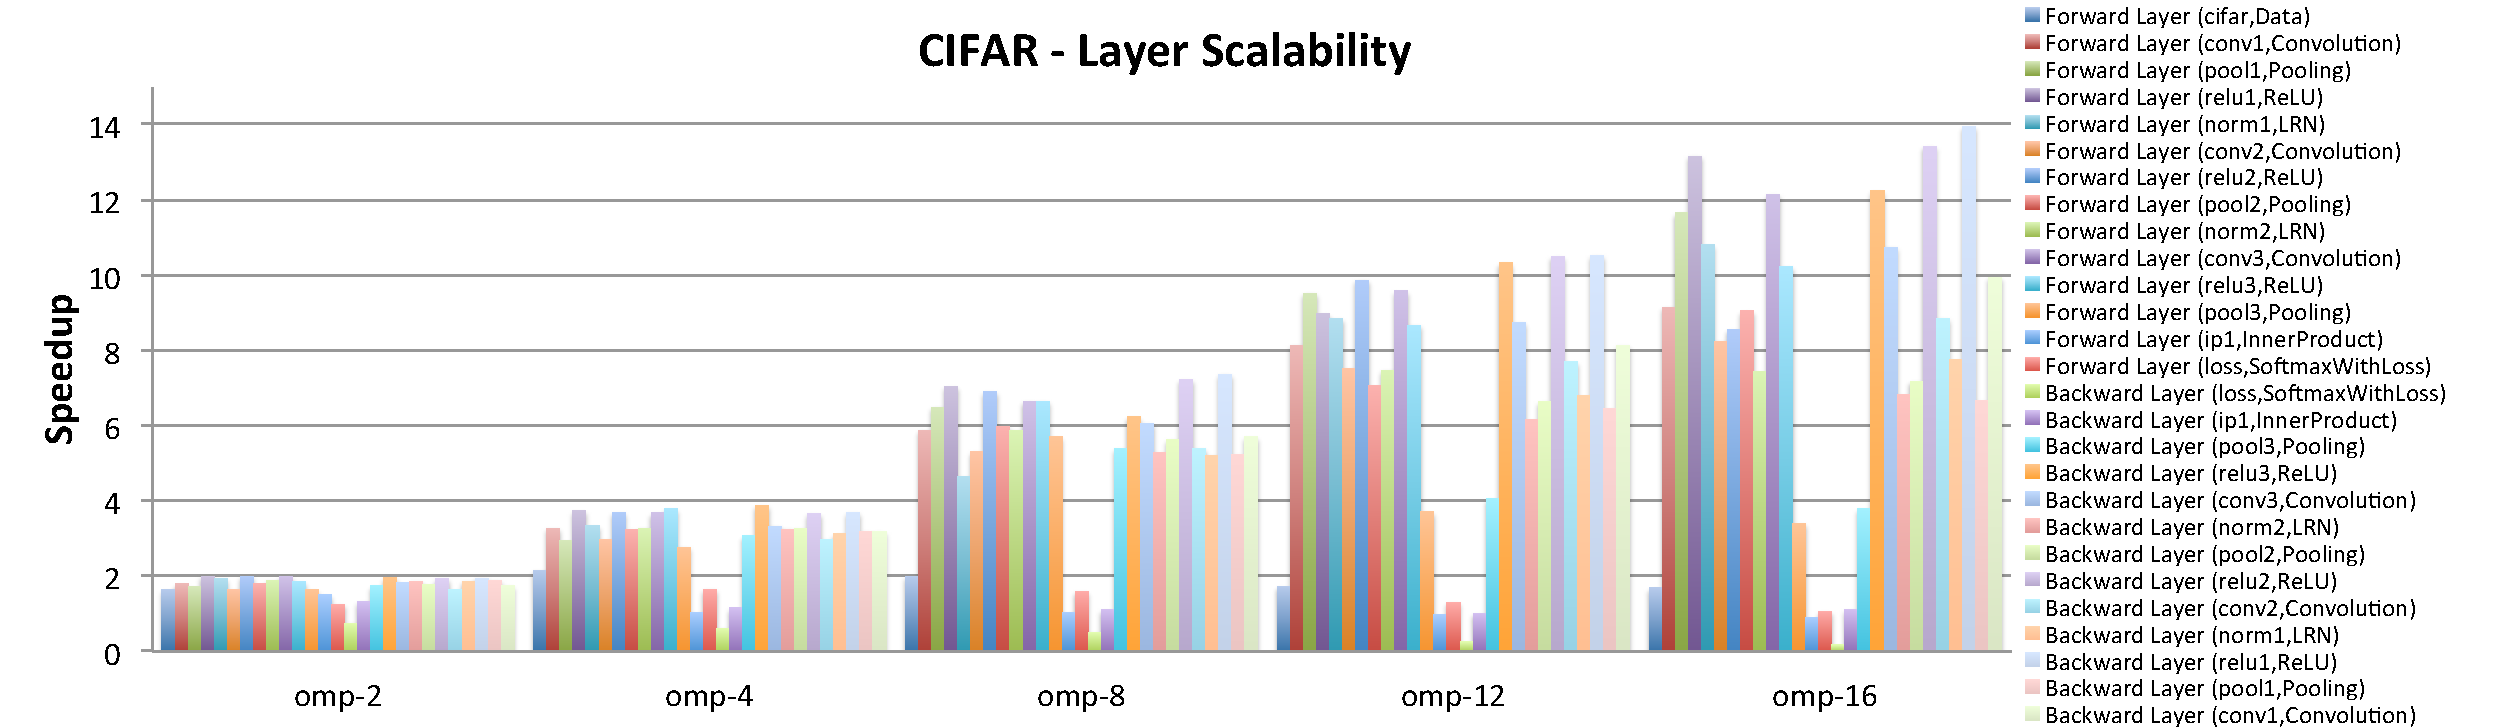
\includegraphics[width=\textwidth]{figures/cifar-scalability-layer.pdf}
\caption{CIFAR-10 - Layer scalability for CPU executions. Layers are identified as in the legend for Figure \ref{fig-cifar-abs-rel}. Layers in the legend are ordered from left-to-right in each cluster. Clusters correspond to the cases of 2, 4, 8, 12 and 16 threads. Y-axis measures speedup factors from the serial CPU execution.}
\label{fig-cifar-scalability}
\end{figure*}

\begin{figure*}[]
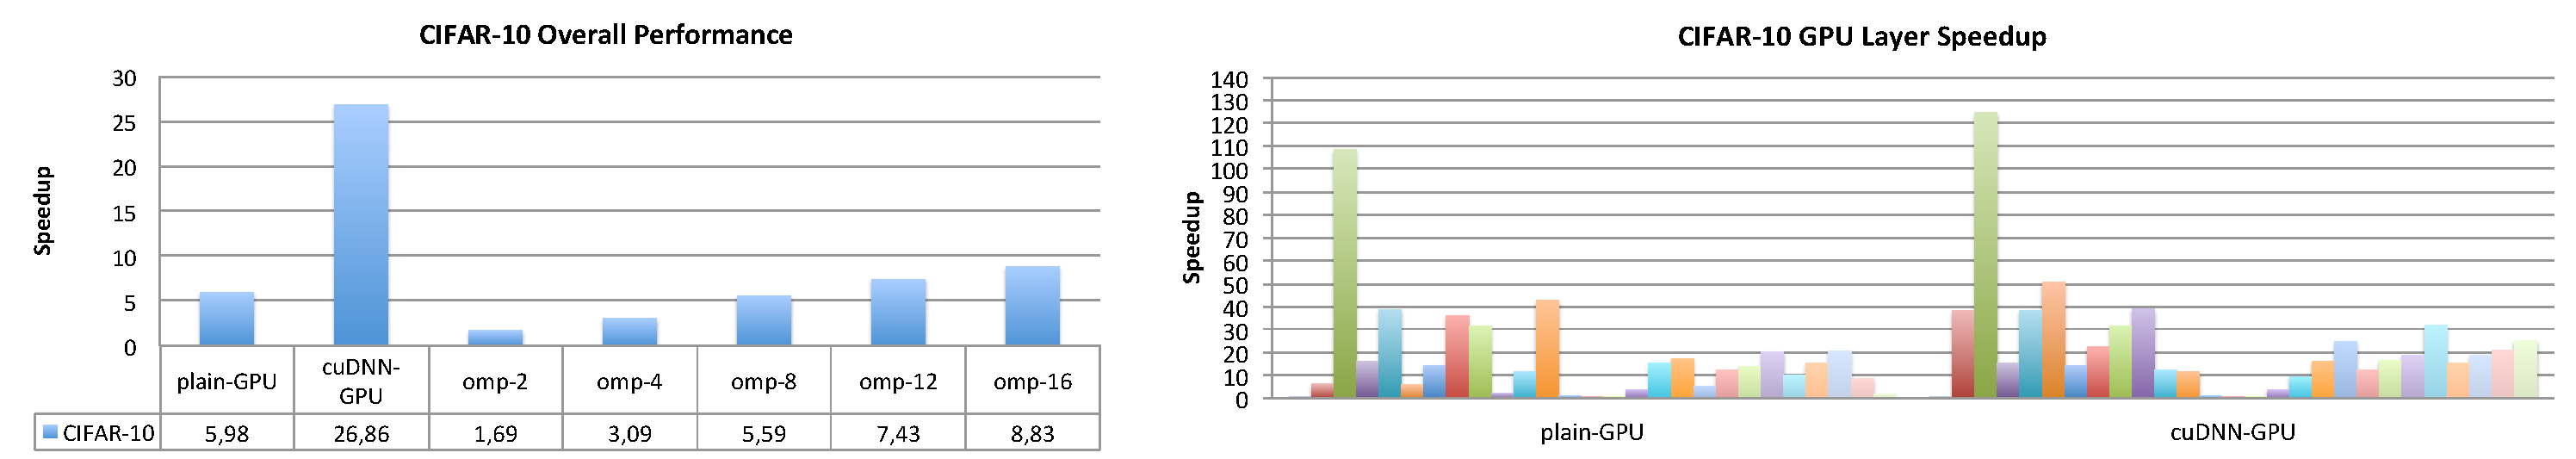
\includegraphics[width=\textwidth]{figures/cifar-abs-perf+gpu-layer.pdf}
\caption{CIFAR-10 - \textbf{Leftmost side}: Absolute speedup factors for OpenMP (2, 4, 8, 12 and 16 threads), plain-GPU and cuDNN-GPU versions. performance. \textbf{Rightmost} side: GPU layer scalability for plain-GPU and cuDNN-GPU versions. Layers are identified as in the legend for Figure \ref{fig-cifar-abs-rel}.}
\label{fig-cifar-overall}
\end{figure*}

\subsection{The CIFAR-10 case}
For the performance analysis of the CIFAR-10 dataset we have followed the 
same methodology as for the MNIST case. First, we have developed a 
per-layer study both coarse-grain and fine-grain parallelizations. 
For the coarse-grain case we identify what are the main limiting 
performance factors. Then we describe the overall performance of the 
coarse-grain parallelization. 

\subsubsection{Coarse-grain Layer Performance}
The CIFAR-10 dataset generates a work granularity greater than 
the MNIST case. This can be observed in Figure \ref{fig-cifar-abs-rel}. 
The figure shows per-layer absolute execution time and the relative 
weight in the overall execution time. It is clear that just a few 
layers dominate the execution, no matter the number of threads. 
These layers are the convolutional and pooling layers, and with 
less weight the local response normalization layers. In general, 
these layers account for almost 85\% of total execution time in 
all thread configurations. Therefore, the layers with very small 
granularity and exposing very poor scalability curves will not 
determine the overall performance. Only the scalability of these 
dominating layers will determine the effectiveness of the 
parallelization.

Figure \ref{fig-cifar-scalability} shows the scalability curves of all layers. 
Notice the appearance of the u-shape form as long as the number of threads 
increases. The center part of each cluster corresponds to layers of very 
small granularity which do not affect the overall performance. These layers 
are the pool3, ip1 and loss. The center part includes both the forward 
and backward pass of these layers. Leftmost part of each cluster 
correspond to the layer forward pass, the rightmost part corresponds 
to the layer backward pass.

The CIFAR-10 network is organized in three levels all of them with a 
similar organization. First level corresponds to a sequence of a data 
layer plus conv1+pool1+ReLU1+norm1. During the forward pass, the data 
layer fetches the input data (e.g: the batch images) sequentially so 
the conv1 layer suffers from poor locality respect its input data 
(the same situation observed with the MNIST case). The work distribution 
is constant across the conv1, pool1 and ReLU1 layers, and then changes 
for the norm1. According to this, the conv1 has a 
reasonable speedup up to 8 threads (5.87$\times$) but for 16 threads the 
scalability drops with a 9$\times$ speedup. This is explained by the 
sequential execution of its immediate previous layer and by the fact 
that when crossing the 8 thread border, NUMA considerations come into 
play. The effects of data movement are much more visible than when 
just executing in one NUMA node. After the conv1 forward execution, 
the pool1 and ReLU1 layers keep the same work distribution and expose 
reasonable speedups: 6.5$\times$ and 7$\times$ respectively with 8 threads. These 
layers scale up to 11$\times$ and 13$\times$ with 16 threads. The norm1 layer exposes 
a different trend. This layer executes changing the data-thread 
distribution. With 8 threads reaches a 4.6$\times$ speedup and with 
16 threads 10.8$\times$. Regarding the backward pass of all the layers 
in this first level, the relation between the layers are similar, 
but with less scalability. The maximum speedup for 16 threads are 
10$\times$, 6.6$\times$, 7.75$\times$ for the conv1, pool1, ReLU1 and norm1 layers respectively. 
The reduction operations within the backward pass are negligible, 
given the work size in each layer for the CIFAR-10 case. This happens 
in all the network levels.

The second level in the network is composed of layers conv2, ReLU2 
and norm2. In this level, the sizes of the input/output blobs decrease 
and the work granularity too, but with the exception of layer conv2. 
This working set size reduction affects the overall scalability, 
specially with 16 threads. In this level, the maximum speedups are 
8.25$\times$, 8.5$\times$, 9$\times$ and 7$\times$. In this case, the data-thread relation between the 
layers is constant, unless for the norm2 layer. Specifically for the 
first layer in this level, the conv2 layer, its poor scalability is 
related to its immediate previous layer, the norm1 layer. This layer 
changes the data-thread distribution and the conv2 layer is affected 
by this fact. For the backward pass, the performance trends are similar, 
and again the reduction operations do not reduce the overall layer 
scalability.

Finally, the third level is composed by the conv3, ReLU3 and pool3 
layers. This level follows a similar performance trends as the second 
level, with the same relations between its layers and between the 
immediate layer in the second level.

%\begin{figure*}[]
%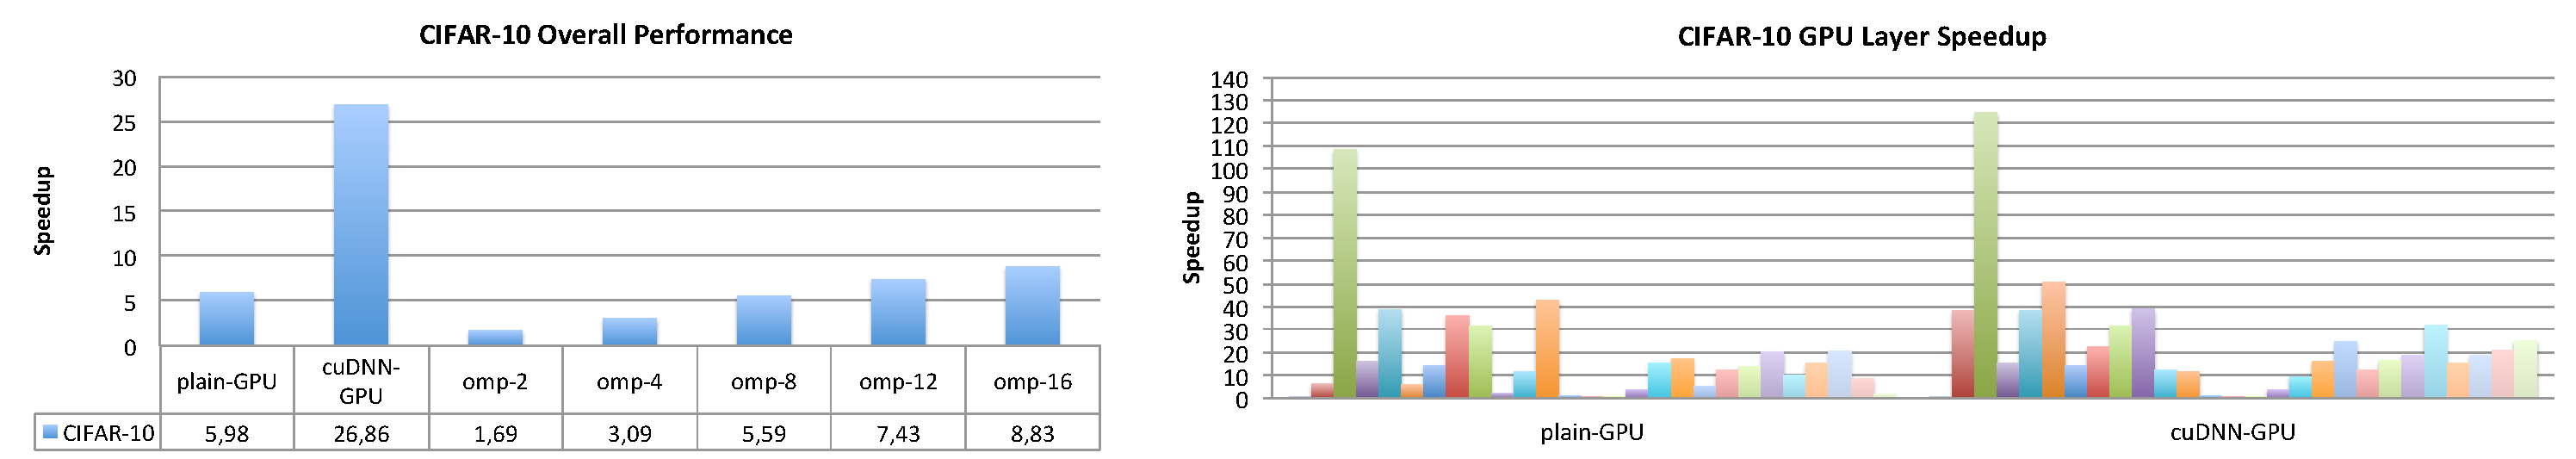
\includegraphics[width=\textwidth]{figures/cifar-abs-perf+gpu-layer.pdf}
%\caption{CIFAR-10 - \textbf{Leftmost side}: Absolute speedup factors for OpenMP (2, 4, 8, 12 and 16 threads), plain-GPU and cuDNN-GPU versions. performance. \textbf{Rightmost} side: GPU layer scalability for plain-GPU and cuDNN-GPU versions. Layers are identified as in the legend for Figure \ref{fig-cifar-abs-rel}.}
%\label{fig-cifar-overall}
%\end{figure*}

\subsubsection{Fine-grain Layer Performance}
Rightmost side of Figure \ref{fig-cifar-overall} shows the per-layer
speedup numbers for the plain-GPU and cuDNN-GPU versions.
For the plain-GPU version, the layer speedups are impressive. 
In the forward pass, all layers present speedups above 10$\times$, and for 
the pooling and LRN layers the speedups are close to 110$\times$ and 40$\times$
respectively (depending on the layer instance and pass in the network). 
The convolutional layers are represent the bottleneck. they present 
speedups between 1.8$\times$ and 6$\times$ depending on the layer position in the 
network and in the pass (forward or backward).

For the cuDNN-GPU, the trends are similar as in the MNISt case 
regarding the convolutional and pooling layers. The convolutional 
layers expose impressive improvements. They switch to performance 
levels close to 50$\times$ of speedup in some cases (conv2 layer).
Some of the pooling layers expose drastic performance drops (pool3 
forward pass switches from 42$\times$ to 11.75$\times$). Others improve the 
performance (pool1 from 8.6$\times$ to 20.9$\times$). 
As it was stated with the MNIST dataset, cuDNN corresponds to a case 
where the industry has deployed a highly optimized implementation of 
specific layer transformations that are well understood and no longer 
in a research stage. In this situation, the fine-grain parallelism makes 
a difference, though after the corresponding recoding efforts.

\subsubsection{Overall Performance}
Figure \ref{fig-cifar-overall} shows the overall performance of
the coarse-grain parallelization and the fine-grain parallelization in
its two versions GPU and GPU-cuDNN. The coarse-grain reaches a speedup
close to a 6$\times$ with 8 threads, and 8.83$\times$ with 16 threads. The lack of
the scalability for the CPU version is related to the poor scalability
of some of the convolutional layers. This is caused by poor data locality caused by consecutive layers with different data-thread patterns. 
In addition, again the serial initialization of
the network structures is giving a suboptimal memory allocation in
the NUMA nodes. All of this is affecting the final scalability of
the coarse-grain version. The fine-grain GPU version shows a
modest speed up close to 6$\times$. Both the fine-grain GPU version and 
coarse-grain CPU version expose problems with the convolutional layers.
In general, the fine-grain GPU version corresponds to the Caffe native 
implementation. This implementation is representative of the 
performance the DNN community can obtain after the associated recoding 
efforts. The coarse-grain parallelization gives similar performance levels, but not requiring the reimplementation of all layers to target the GPU device. 
As with the MNIST case, when compared to the cuDNN case, the fine-grain 
approach makes a difference and this time even greater. cuDNN gives 
extraordinary speedups and it corresponds to an unbeatable implementation 
of the convolutional and pooling layers made by NVIDIA. It delivers a 
27$\times$ speedup. Unfortunately, this performance levels are only available 
for these two layer types. In contrast, the coarse-grain approach is 
immediately available no matter the nature of the deep neural network.

\subsection{Coarse-grain vs Fine-grain: Pros and Cons}
In this section we present the lessons learnt regarding the coarse-grain 
and fine-grain parallelizations of the DNN training process. We identify 
several limiting factors that affect the performance of the 
coarse-grain parallelization. These factors are layer dependent and are 
mainly related to specificities of the layers that determine their 
work distribution, memory footprint, data privatization and ordered 
operations. Also, we identify the advantages and disadvantages of 
the coarse-grain approach in front a fine-grain parallelization. 
The following paragraph describes these limiting factors, 
advantages and disadvantages.

\textbf{Network agnostic}: one important advantage of the coarse-grain 
approach is that it exploits a parallelism level that is independent of 
the nature of the neural network. The batch-level parallelism is 
intrinsic to the gradient descent algorithm. Thus, this approach is 
immediately available and does not require programming efforts to generate 
GPU layer implementations. In addition, the coarse-grain approach 
delivers similar performance levels as the fine-grain approach. 
\textbf{Convergence invariance}: the coarse-grain parallelization does not 
change any training parameters. Thus, the convergence rate is kept 
invariant between the serial and the parallel executions. 
For the DNN community this is an important advantage. Before 
the training, neural networks need a parameter tuning process to ensure 
appropriate convergence. The parallelization has to ensure that the effects of this tuning are kept for the parallel execution.
\textbf{Sequential memory allocation}: the network memory allocation
happens during the network initialization. This process is sequential, 
which causes the layer memory be allocated following a
pattern generated by the initialization code. In terms of performance, 
this pattern is not compatible with those that arise during
the training process.
\textbf{Locality between layers:} the input/output relation across layers
defines a lost of data locality for specific layers. During the forward 
and backward passes, each layer distributes the work according to the 
dimensions of the input blobs. Regarding the data locality, it is 
possible that input and output blobs do not match
their dimensions. Consequently, the work distribution and data-thread
association defined in one layer will not match that one of the
next immediate layer in the stack.
One particular case of this situation corresponds to the data
layers in Caffe. These layers feed the network with input data
organized in batches. Data layers execute in sequentially.
Therefore, a one thread first accesses all data and then the data is
distributed across the cores and the memory hierarchy when the
first parallel processing layer in the network is executes in parallel. 
\textbf{Work unbalance:} coarse grain parallelism is open to work unbalance. 
For the Caffe case, we have detected that batch-level parallelism 
defines very heavy iterations for the parallelized loops.
Therefore, one single loop iteration can cause a high unbalance
between the executing threads. Loop coalescing has been applied to reduce the effect of this problem.
\textbf{Work granularity:} neural networks do
a dimensionality reduction over the processed data.
And this affects the size of the working sets in the network layers.
At some level in the network, the input/output blobs start decreasing their sizes. When this happens, a thread level parallelization
starts suffering from too small work granularity with poor performance levels.
\textbf{Data privatization and reduction operations:} specifically in the
backward pass, the network coefficients are updated per each
sample in the batch. At batch-level, this requires mutual exclusion
mechanisms to guarantee a ordered update. Data privatization has
been needed for this purpose. In terms of performance, given the 
layer granularity, we have not detected these updates to be a 
performance limiting factor.


